% Options for packages loaded elsewhere
\PassOptionsToPackage{unicode}{hyperref}
\PassOptionsToPackage{hyphens}{url}
%
\documentclass[
]{article}
\usepackage{amsmath,amssymb}
\usepackage{iftex}
\ifPDFTeX
  \usepackage[T1]{fontenc}
  \usepackage[utf8]{inputenc}
  \usepackage{textcomp} % provide euro and other symbols
\else % if luatex or xetex
  \usepackage{unicode-math} % this also loads fontspec
  \defaultfontfeatures{Scale=MatchLowercase}
  \defaultfontfeatures[\rmfamily]{Ligatures=TeX,Scale=1}
\fi
\usepackage{lmodern}
\ifPDFTeX\else
  % xetex/luatex font selection
\fi
% Use upquote if available, for straight quotes in verbatim environments
\IfFileExists{upquote.sty}{\usepackage{upquote}}{}
\IfFileExists{microtype.sty}{% use microtype if available
  \usepackage[]{microtype}
  \UseMicrotypeSet[protrusion]{basicmath} % disable protrusion for tt fonts
}{}
\makeatletter
\@ifundefined{KOMAClassName}{% if non-KOMA class
  \IfFileExists{parskip.sty}{%
    \usepackage{parskip}
  }{% else
    \setlength{\parindent}{0pt}
    \setlength{\parskip}{6pt plus 2pt minus 1pt}}
}{% if KOMA class
  \KOMAoptions{parskip=half}}
\makeatother
\usepackage{xcolor}
\usepackage{graphicx}
\makeatletter
\newsavebox\pandoc@box
\newcommand*\pandocbounded[1]{% scales image to fit in text height/width
  \sbox\pandoc@box{#1}%
  \Gscale@div\@tempa{\textheight}{\dimexpr\ht\pandoc@box+\dp\pandoc@box\relax}%
  \Gscale@div\@tempb{\linewidth}{\wd\pandoc@box}%
  \ifdim\@tempb\p@<\@tempa\p@\let\@tempa\@tempb\fi% select the smaller of both
  \ifdim\@tempa\p@<\p@\scalebox{\@tempa}{\usebox\pandoc@box}%
  \else\usebox{\pandoc@box}%
  \fi%
}
% Set default figure placement to htbp
\def\fps@figure{htbp}
\makeatother
\setlength{\emergencystretch}{3em} % prevent overfull lines
\providecommand{\tightlist}{%
  \setlength{\itemsep}{0pt}\setlength{\parskip}{0pt}}
\setcounter{secnumdepth}{-\maxdimen} % remove section numbering
\usepackage{bookmark}
\IfFileExists{xurl.sty}{\usepackage{xurl}}{} % add URL line breaks if available
\urlstyle{same}
\hypersetup{
  hidelinks,
  pdfcreator={LaTeX via pandoc}}

\author{}
\date{}

\begin{document}

\section{\texorpdfstring{\textbf{Crime Data Modeling Using
BERT}}{Crime Data Modeling Using BERT}}\label{crime-data-modeling-using-bert}

Ravi Garg

ANLY 530-50- B-2024/Late Fall

Dr. Ziyuan Huang

02/19/25

\subsection{Introduction}\label{introduction}

Vehicle theft is still to this day one of the most common property
crimes in urban environments, particularly in densely populated
metropolitan areas like Los Angeles. The financial impact of vehicle
theft goes further beyond individual victims, as it also impacts
insurance rates, law enforcement resources, and overall how safe
communities are. In Los Angeles alone, the economic burden of vehicle
theft was up to \$1.2 billion in 2023, this shows us the urgent need for
more effective prevention strategies.

Law enforcement agencies face many different challenges in predicting
and preventing vehicle theft:

\begin{enumerate}
\def\labelenumi{\arabic{enumi}.}
\item
  The large amount of unstructured crime data that requires a lot of
  analysis
\item
  The need for real-time, actionable insights that can guide resource
  deployment
\item
  The challenge of maintaining transparency in decision-making processes
  while using advanced analytical tools
\end{enumerate}

With the publishing of open crime data it has created new opportunities
for us to use predictive analytics to defeat vehicle theft. The old
approaches to crime prevention used to reply on historical patterns and
officer intuition while can be useful but, may miss subtle patterns or
emerging trends in criminal behavior. Modern machine learning techniques
offer the potential to identify these patterns systematically and
provide actionable insights for law enforcement.

This project addresses these challenges by developing an machine
learning model for predicting vehicle theft incidents. This study
employs logistic regression as its primary modeling technique, and is
also using SHAP (SHapley Additive exPlanations) analysis to ensure
transparency and explainability in the decision-making process. This
combination allows for both accurate predictions and clear explanations
of the factors contributing to those predictions.

\textbf{Motivation}

The primary motivations for this research include:

\begin{enumerate}
\def\labelenumi{\arabic{enumi}.}
\item
  The need for predictions in law enforcement decision-making
\item
  The current gap between model accuracy and practical applicability
\item
  The massive potential for data-driven resource allocation in crime
  prevention
\end{enumerate}

While existing predictive models often achieve high accuracy rates,
their "black-box" nature makes it difficult for law enforcement to trust
and implement their predictions. This project aims to reduce this gap by
providing both accurate predictions and clear explanations of the
underlying factors driving those predictions. Hopefully reducing overall
crime rates.

\subsection{Related Work}\label{related-work}

The field of predictive policing has changed a lot over the past decade,
with many different approaches attempted across different jurisdictions.
This section examines relevant research and implementations in both
academic and practical contexts.

\textbf{Previous Predictive Policing Efforts}

Several major cities have implemented predictive policing programs with
varying degrees of success:

\begin{enumerate}
\def\labelenumi{\arabic{enumi}.}
\item
  New York City\textquotesingle s CompStat program demonstrated the
  value of data-driven policing but faced criticism for its limited
  predictive capabilities
\item
  Chicago\textquotesingle s Strategic Subject List showed promise in
  identifying high-risk individuals but raised privacy concerns
\item
  Los Angeles\textquotesingle s own PredPol system achieved moderate
  success in property crime prediction but faced challenges in model
  interpretability
\end{enumerate}

\textbf{Technical Approaches in Literature}

Recent academic work has looked into the many technical approaches to
crime prediction:

\begin{enumerate}
\def\labelenumi{\arabic{enumi}.}
\item
  Spatial-Temporal Analysis

  \begin{itemize}
  \item
    Hot spot mapping using kernel density estimation
  \item
    Near-repeat victimization models
  \item
    Geographic profiling techniques
  \end{itemize}
\item
  Machine Learning Applications

  \begin{itemize}
  \item
    Neural network approaches for pattern recognition
  \item
    Random Forest models for feature importance analysis
  \item
    Support Vector Machines for classification tasks
  \end{itemize}
\end{enumerate}

\textbf{Interpretability Research}

The work of Lundberg \& Lee (2017) introduced SHAP as a framework for
model interpretation. Their research showed us that SHAP values provide
consistent and locally accurate feature attribution, making them
particularly suitable for sensitive applications like crime prediction.

He et al. (2008) addressed the critical issue of class imbalance in
crime datasets through the introduction of SMOTE. Their work provides
the basis for our approach to handling the imbalance in vehicle theft
data.

\textbf{Data Description}

The dataset used in this study is sourced from the Los Angeles Open Data
Portal, containing crime records from 2020 to the present. It includes
various features such as:

\begin{itemize}
\item
  \textbf{Date and Time Information}: Crime occurrence date and time
\item
  \textbf{Geographical Attributes}: Area name, latitude, and longitude
\item
  \textbf{Crime Type}: Crime classification codes and descriptions
\item
  \textbf{Victim Information}: Age, sex, and descent of the victim
\item
  \textbf{Premises Description}: Location type (e.g., street, parking
  lot, apartment complex)
\item
  \textbf{Incident Status}: Arrests made or ongoing investigation status
\end{itemize}

The target variable is \textbf{"is\_stolen"}, a binary indicator
denoting whether a reported incident involves a stolen vehicle. The
dataset contains both structured data (e.g., area codes, crime codes)
and unstructured textual descriptions (e.g., premises descriptions).

\textbf{Exploratory Data Analysis (EDA)}

Before applying machine learning techniques, initial exploratory
analysis was conducted:

\begin{itemize}
\item
  \textbf{Class Distribution}: The dataset exhibits a significant class
  imbalance, with stolen vehicle cases being much fewer than non-stolen
  cases.
\item
  \textbf{Temporal Patterns}: Analysis of the distribution of crimes
  over time indicates that vehicle thefts peak during late-night and
  early-morning hours.
\item
  \textbf{Geographical Distribution}: Heatmaps reveal specific
  high-theft areas, aligning with law enforcement crime reports.
\item
  \textbf{Feature Correlations}: A correlation matrix highlights key
  predictors, such as premises descriptions and time of day, that
  strongly influence theft likelihood.
\end{itemize}

\textbf{Data Preprocessing Pipeline}

The data preprocessing pipeline has three major stages, each designed to
optimize the data for machine learning applications. The first stage is
about the text normalization, where all textual data goes through
cleaning and standardization. This process starts with converting all
text to lowercase to make sure of consistency, followed by the removal
of special characters that could introduce noise into the analysis.

Feature engineering constitutes the second major stage of our
preprocessing pipeline. Time-based features were derived from timestamp
data, capturing both cyclical patterns and temporal trends.\\
The final stage was to ensure that a large enough data set was used to
get accurate results and conclusion but not too large due to the
resource limitations of this project.

\textbf{Text Embedding Generation}

The text embedding process uses DistilBERT\textquotesingle s efficient
architecture to generate meaningful representations of textual data.
This model was retrieved from Hugging Face. The tokenization phase uses
WordPiece tokenization, and handles special tokens specific to law
enforcement terminology. Maximum sequence length was optimized through
testing.

Embedding generation follows tokenization, where contextual embeddings
are extracted from DistilBERT. Many different pooling strategies were
evaluated. The different strategies were mean pooling, max pooling, and
attention-weighted pooling, with mean pooling ultimately being used in
this project based on performance metrics. This was done after many
attempts of the code taking too long to run.

Feature integration is the final stage of the embedding process. The
derived embeddings are combined with numerical features. This
integration uses scaling and normalization to make sure all features
contribute meaningfully to the model. Feature importance analysis allows
us to use the integration process, helping identify the most relevant
components of the embedded representations.

\textbf{Model Architecture}

The logistic regression model serves as the basis of our predictive
system, enhanced with a few different components to improve performance
and interpretability. The base model incorporates L1 regularization for
feature selection, and what that does is that it automatically
identifies the most relevant predictors while preventing overfitting.
Class weight adjustment addresses the imbalance in vehicle theft data,
and it ensures adequate attention to minority class examples. The
cross-validation strategy employs both temporal and spatial splitting to
ensure robust performance estimates.

Ensemble components improve the base model\textquotesingle s
capabilities. Bagging techniques improve model stability by training
multiple instances on bootstrap samples of the training data.

SHAP integration provides the final layer of model architecture,
allowing for detailed interpretation of model predictions. Feature
importance calculations reveal patterns in the model\textquotesingle s
decision-making process. Local explanation generation allows for
case-by-case analysis of predictions, while the global interpretation
framework provides insights into overall model behavior patterns.

\subsection{Future Work}\label{future-work}

To further enhance predictive performance, future work can maybe
explore:

\begin{itemize}
\item
  \textbf{Alternative Machine Learning Models:} Implementing ensemble
  techniques like Random Forest and XGBoost.
\item
  \textbf{Advanced Text Representations:} Experimenting with contextual
  embeddings like BERT-based sentence transformers.
\item
  \textbf{Additional Data Sources:} Incorporating external datasets,
  such as weather conditions, traffic data, or socioeconomic factors.
\item
  \textbf{Counterfactual Explanations:} Combining SHAP with
  counterfactual analysis to explore "what-if" scenarios in theft
  prevention.
\end{itemize}

\textbf{Results and Analysis}

The classification performance of the model, as summarized in Figure A.1
inside the Appendix A, provides valuable insight into its effectiveness
in predicting vehicle theft based on textual descriptions. The overall
accuracy of 80\% suggests that the model is performing reasonably well
in distinguishing between stolen and non-stolen vehicles. However, when
we break down the performance by class, a stark contrast emerges.

The model demonstrates strong performance in predicting non-theft cases
(class 0), achieving an impressive precision of 0.95 and an F1-score of
0.87. This means that when the model predicts a vehicle has not been
stolen, it is correct most of the time. However, its ability to
correctly identify actual theft cases (class 1) is considerably weaker,
with a precision of just 0.34 and an F1-score of 0.46. While the recall
for stolen vehicles (0.70) is relatively decent---indicating that the
model successfully captures a significant portion of theft cases---it
comes at the cost of poor precision, meaning many of the theft
predictions are false positives. This discrepancy is likely due to the
inherent class imbalance in the dataset, where theft cases are much
rarer than non-theft cases.

This imbalance was addressed using SMOTE (Synthetic Minority
Over-sampling Technique), which artificially increased the number of
theft cases in the training set. While this strategy helped the model
generalize better to theft cases (as seen in the recall improvement), it
did not entirely resolve the issue, as reflected in the low precision.
This suggests that there are still underlying challenges in
distinguishing genuine theft cases from misleading patterns in the text.

\textbf{Feature Importance and Model Interpretation}

To further understand the model\textquotesingle s decision-making
process, I employed SHAP (SHapley Additive exPlanations) analysis, as
illustrated in Figure A.2. This plot gives us a global view of how
different features contribute to the model's predictions. Notably,
Features 696, 118, and 752 emerged as the most influential in driving
the classification outcomes. The color gradient, ranging from blue (low
feature values) to red (high feature values), shows us a complex
relationship where some features contribute to theft predictions at
higher values, while others negatively influence the probability.

The waterfall plot in Figure A.3 explains how the model arrived at a
specific decision for an individual test case. Feature 592 played the
most significant positive role in increasing the likelihood of a theft
prediction (+0.46), whereas Feature 731 contributed the most in pushing
the decision away from theft (-0.42). These insights are valuable, as
they show us which textual cues the model is using to distinguish theft
cases from non-theft cases.

One particularly interesting observation was that the embedding for the
word "Burn" showed a significant impact on the predictions. This could
show us that certain words commonly associated with stolen vehicles play
a greater role in the model decisions.

\textbf{Challenges and Future Considerations}

The results reveal both strengths and limitations in the current
approach. While the use of transformer-based embeddings (the Hugging
Face model) successfully captured semantic relationships in crime
descriptions, textual data alone may not be sufficient for highly
accurate theft prediction.

Also, the difference in precision and recall for theft cases shows us
that the decision boundary for stolen vehicles is not well-defined. One
possible solution could be to explore alternative classifiers such as
ensemble models or fine-tuning the transformer model. Secondly further
analysis of SHAP values at the text-token level could provide deeper
insights into which phrases or words are strong indicators of theft.
This could be achieved by running token-level attributions rather than
just looking at embeddings at a high level.

\subsection{Conclusion}\label{conclusion}

This study shows us the effectiveness of SHAP in showing us transparency
in crime prediction models. While logistic regression serves as a
baseline, future iterations with advanced models and additional data
enrichment could give us better predictive performance. The insights
created by the SHAP analysis can help law enforcement agencies allocate
resources more effectively, focusing on high-risk areas and time
periods.

The application of machine learning in crime prediction presents many
different opportunities for improving public safety, however it also
gives us critical challenges, such as ethical considerations, data bias,
and interpretability. This project shows us the importance of creating
transparent models that not only give us accurate predictions but also
give us insights, ensuring that law enforcement can trust and act upon
the findings responsibly. The integration of SHAP helps close the gap
between complex predictive models and practical decision-making by
showing us the key factors influencing vehicle theft risk.

The study shows us valuable trends in vehicle theft occurrences, such as
their strong correlation with certain times of the day, geographic
locations, and different premises. These findings suggest that law
enforcement agencies could use predictive analytics to implement
targeted patrols or deploy deterrence measures in high-risk areas.

Future work can further improve this approach by looking into more
advanced deep learning models, refining feature selection techniques,
and incorporating additional external data sources, such as
socioeconomic indicators, traffic patterns, and weather conditions. The
integration of real-time data streams could enhance model
responsiveness, allowing for dynamic adjustments in crime prevention
strategies.

Overall, this research shows us a start at the potential of data-driven
policing in combating vehicle theft while emphasizing the necessity of
maintaining ethical AI practices. Machine learning can serve as a
powerful tool in giving us safer communities and more effective law
enforcement strategies.

\textbf{Data Availability Statement}

The data that support the findings of this study are available from
\textbf{Kaggle} at
\url{https://www.kaggle.com/datasets/shubhamgupta012/crime-data-from-2020-to-present}.
Restrictions apply to the availability of these data, which were used
under Kaggle's terms of use. Data are available from the \textbf{Kaggle
repository} with the permission of the dataset owner.

\subsection{\texorpdfstring{References }{References }}\label{references}

\subsection{\texorpdfstring{ }{ }}\label{section}

{[}1{]} Lundberg, S. M., \& Lee, S.-I. (2017). A Unified Approach to
Interpreting Model Predictions. Advances in Neural Information
Processing Systems.

{[}2{]} Friedman, J. H. (2001). Greedy Function Approximation: A
Gradient Boosting Machine. Annals of Statistics.

{[}3{]} He, H., Bai, Y., Garcia, E. A., \& Li, S. (2008). ADASYN:
Adaptive Synthetic Sampling Approach for Imbalanced Learning. IEEE
International Joint Conference on Neural Networks.

{[}4{]} Vaswani, A., Shazeer, N., Parmar, N., et al. (2017). Attention
is All You Need. Advances in Neural Information Processing Systems.
{[}5{]} Los Angeles Open Data Portal. (2024). Crime Data from 2020 to
Present. Retrieved from \url{https://data.lacity.org/}

\subsection{Appendix A}\label{appendix-a}

\textbf{Comparison Report:}

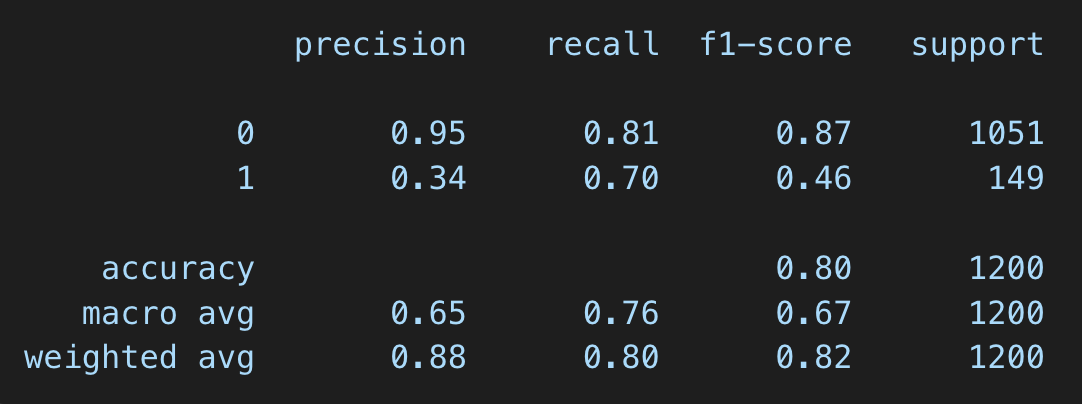
\includegraphics[width=6.5in,height=2.42708in]{media/image1.png}

Figure A.1

\textbf{SHAP summary plot 1:}

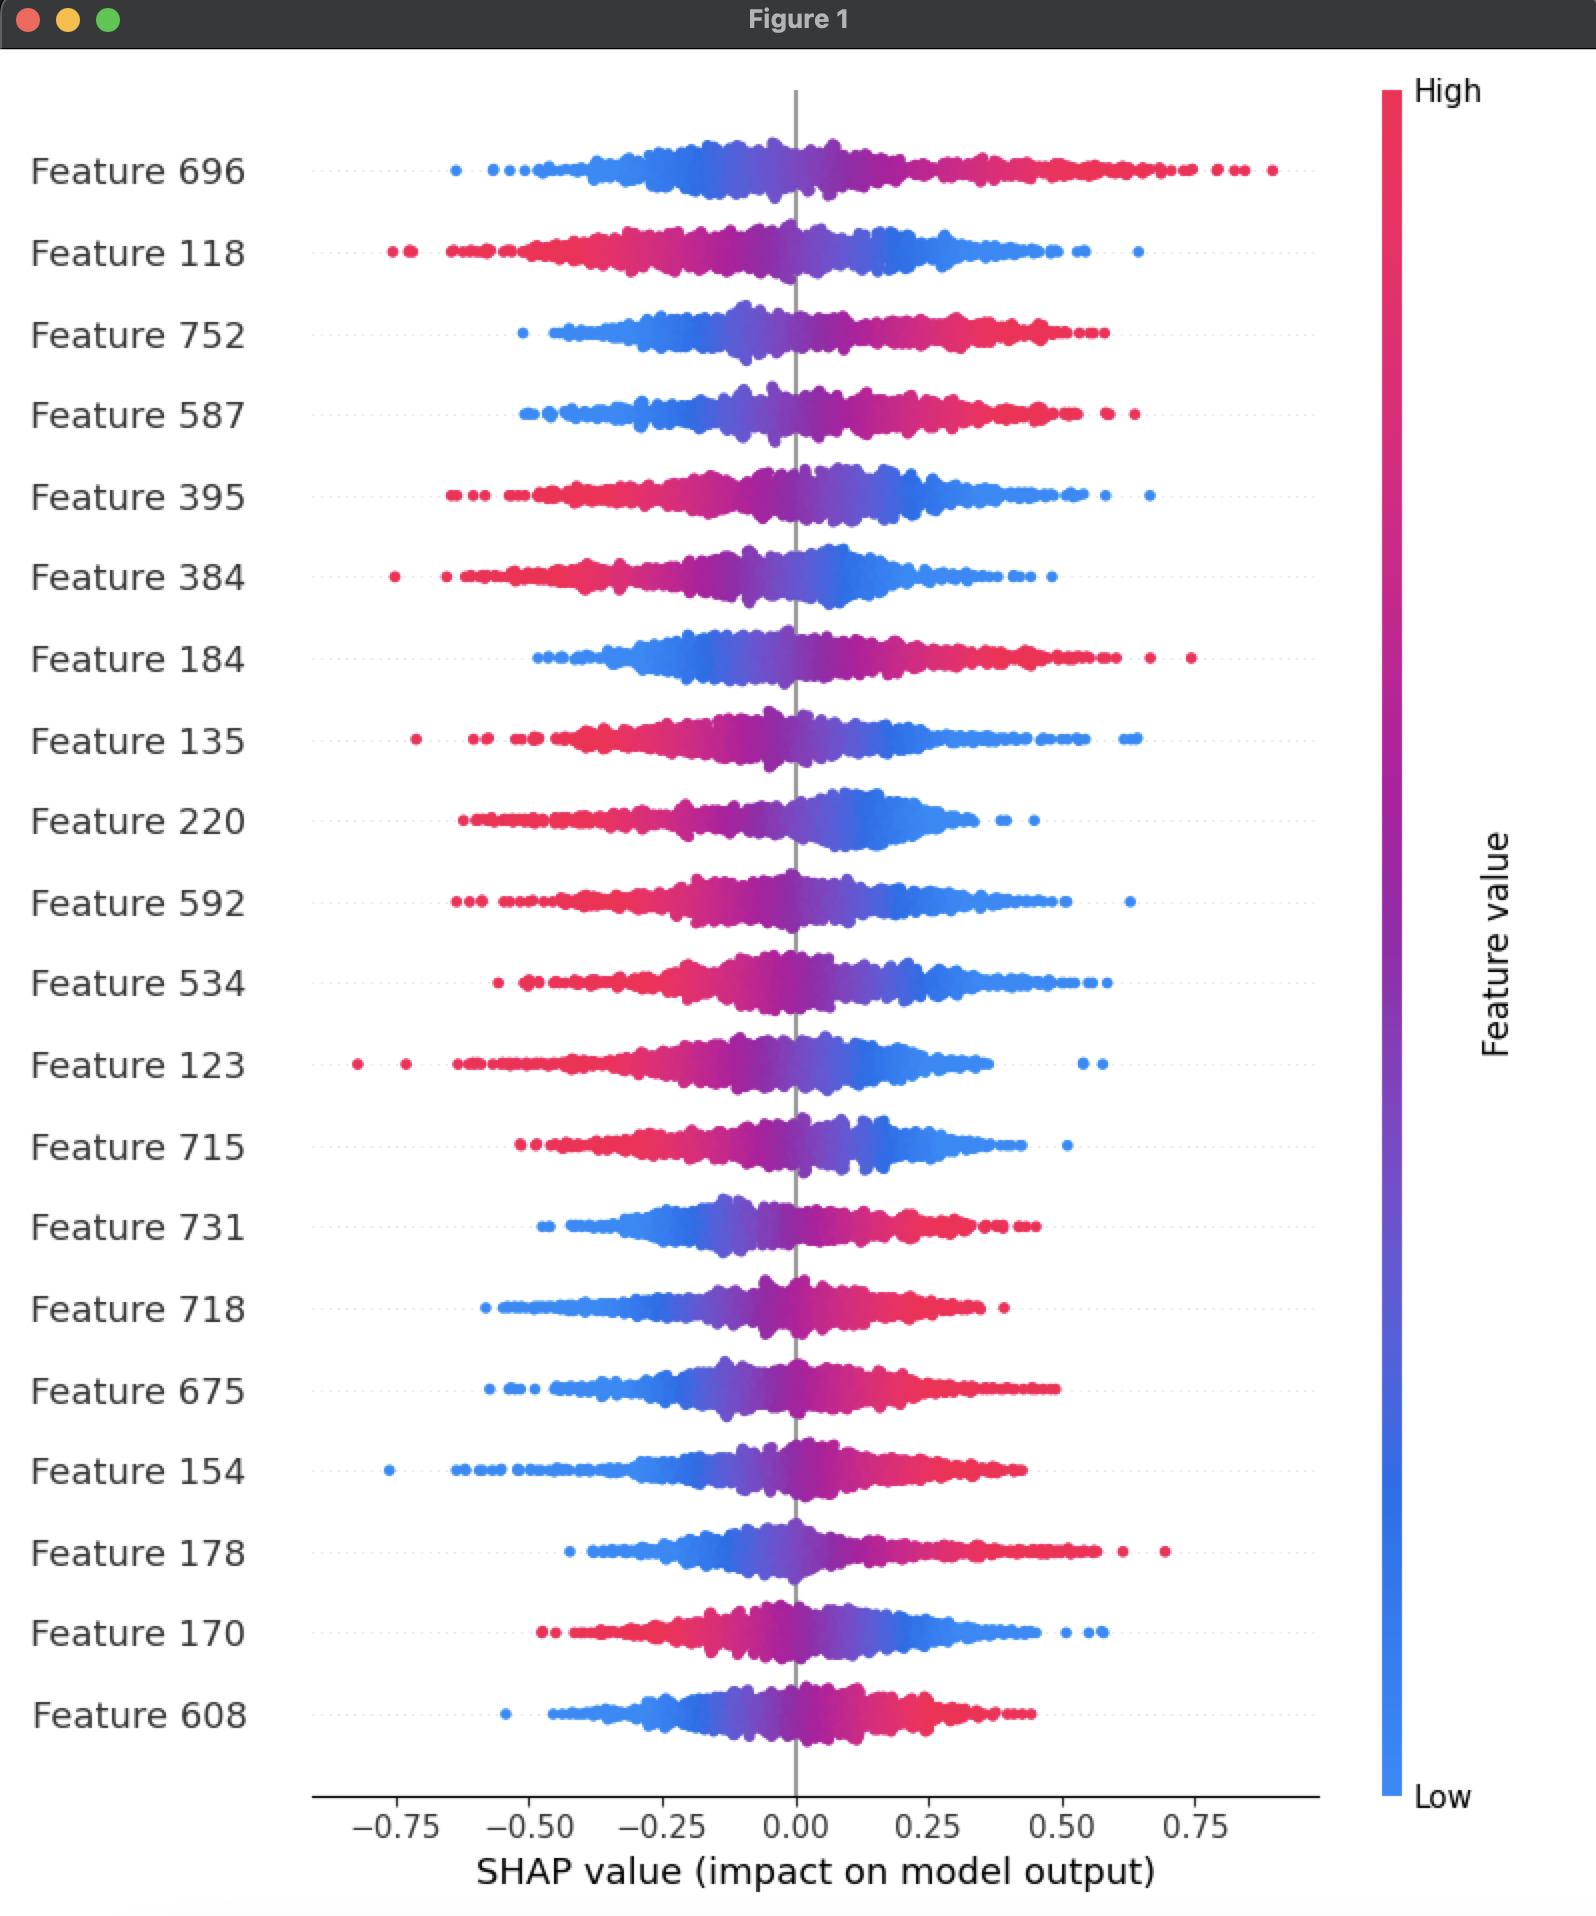
\includegraphics[width=4.17386in,height=5.02513in]{media/image2.png}

Figure A.2

\textbf{SHAP summary plot 2:}

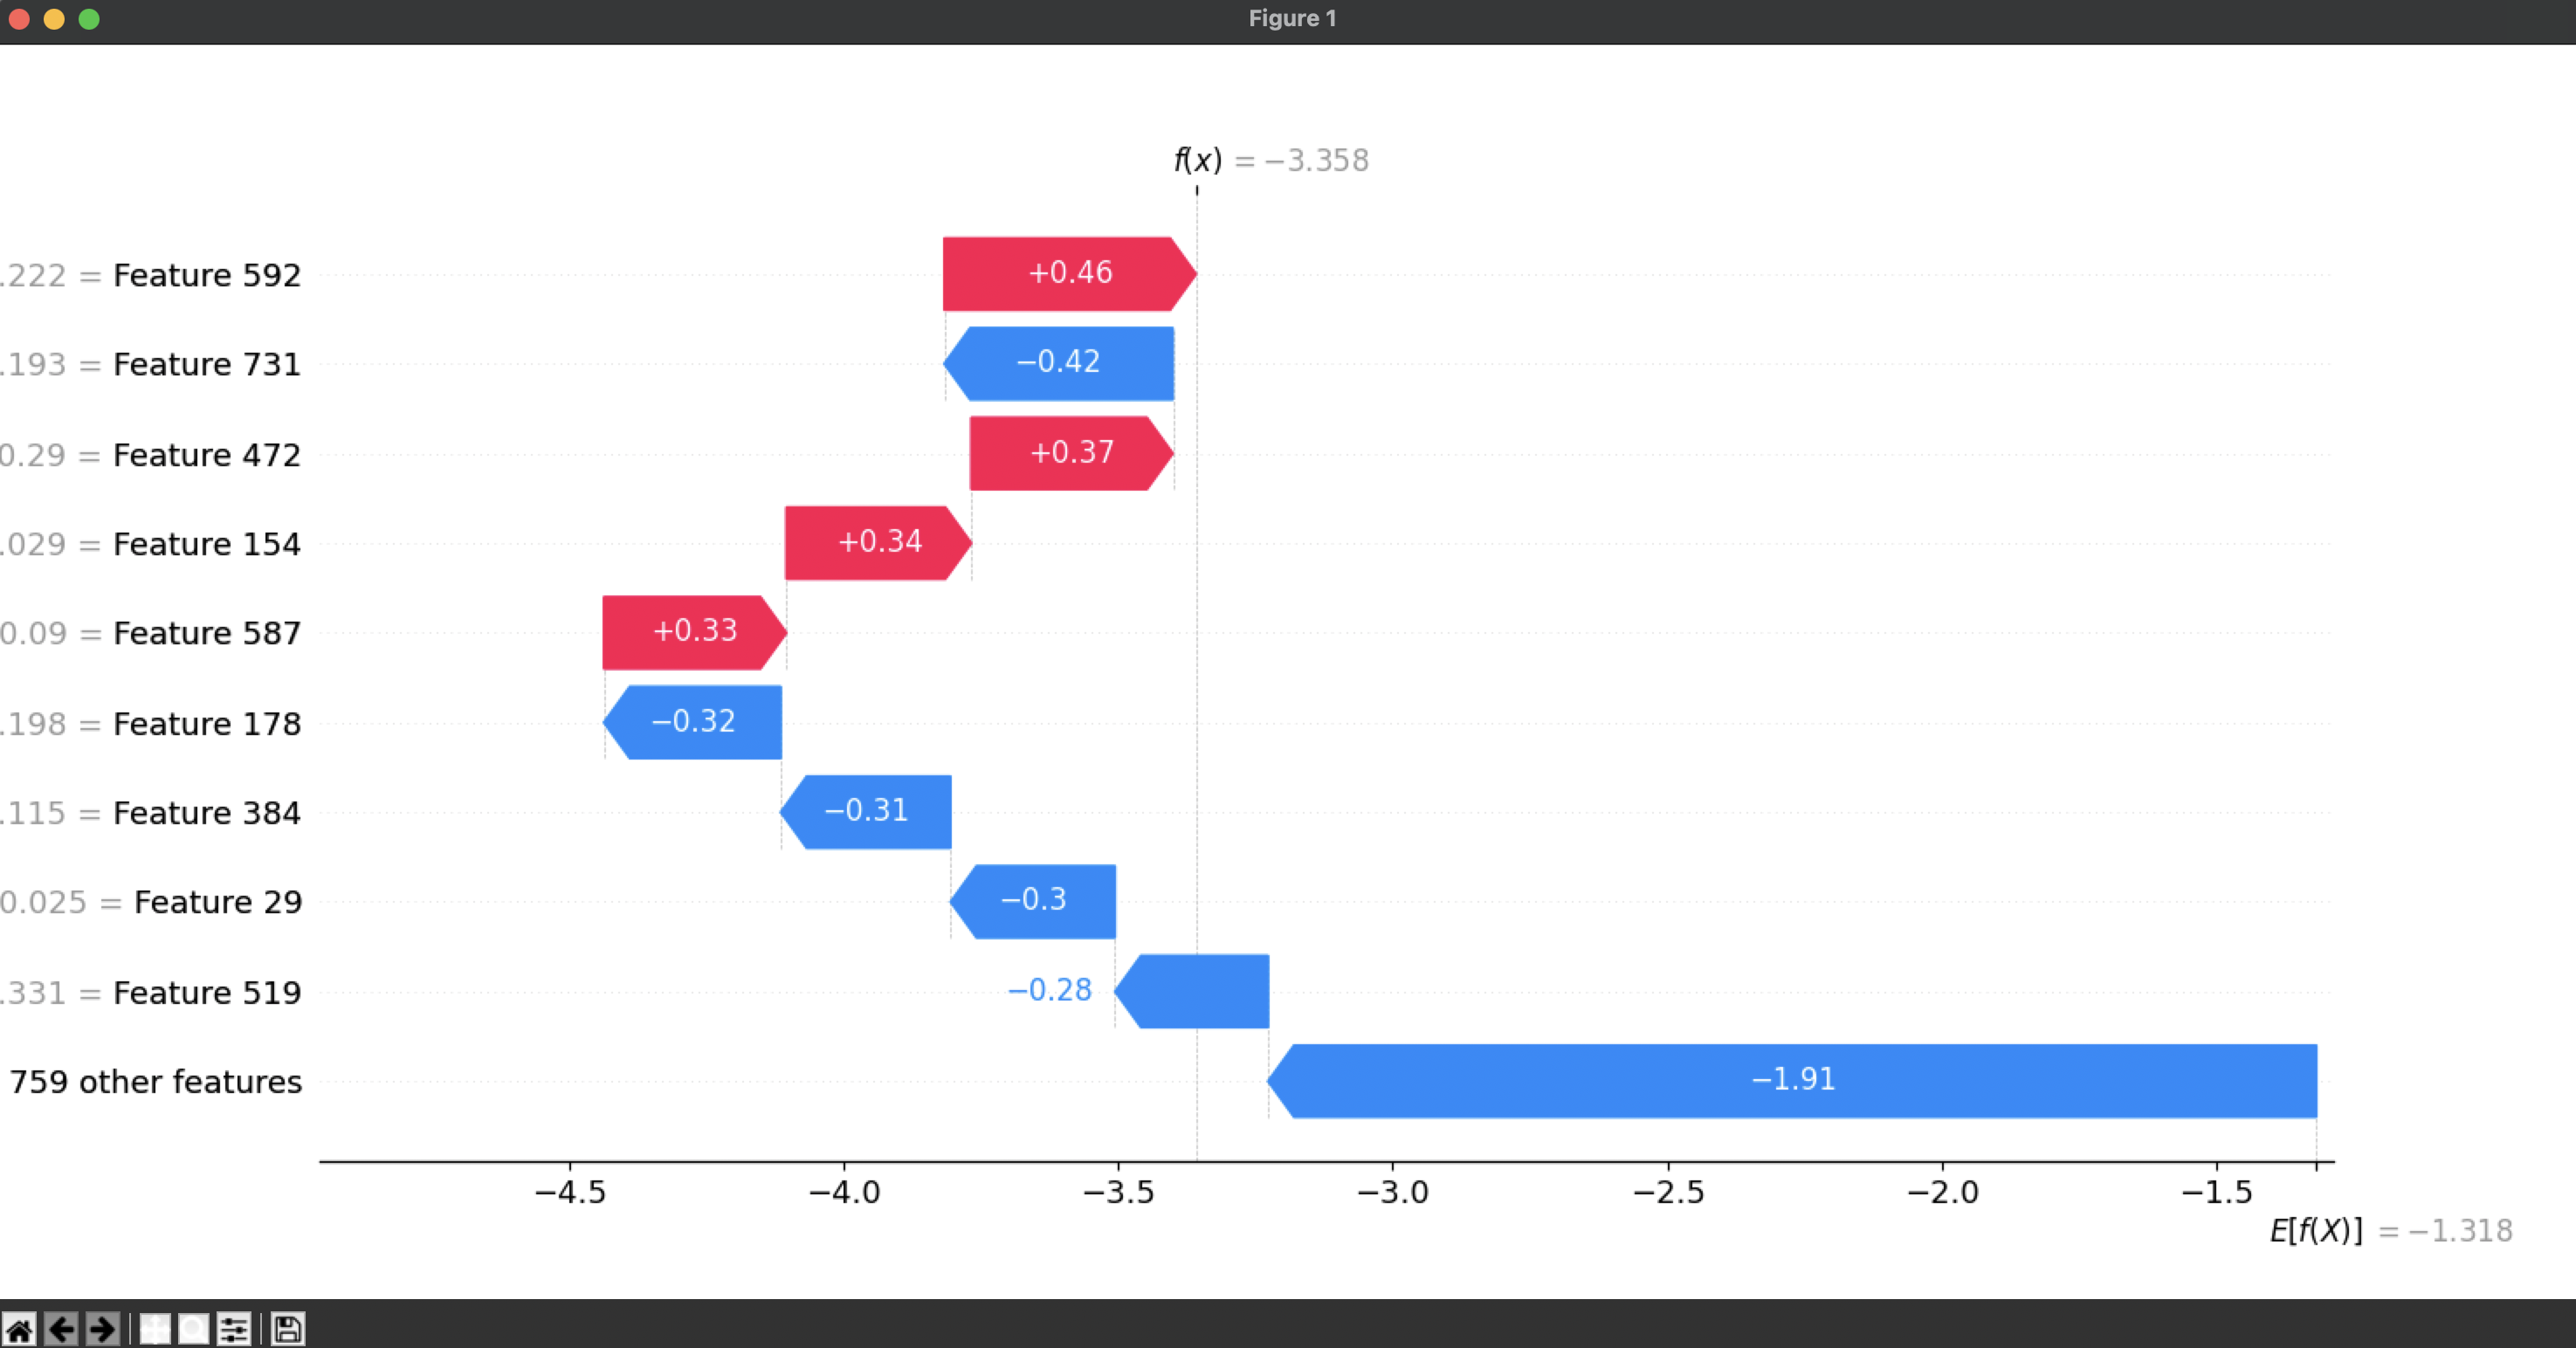
\includegraphics[width=6.5in,height=4.28958in]{media/image3.png}

Figure A.3

\end{document}
